\documentclass[../thesis.tex]{subfiles}
\begin{document}
\chapter{Overview of Organic Semiconductors}

\section{Organic Semiconductors}

Organic molecules are broadly classified as molecules containing carbon.\cite{Pope1999}.
These molecules can range dramatically in size, and are often split into small molecule ($m_w<1$ kg/mol) and polymers.
For organic electronics, molecular semiconductars are of the most interest.

\begin{wrapfigure}{r}{.5\textwidth}
\centering
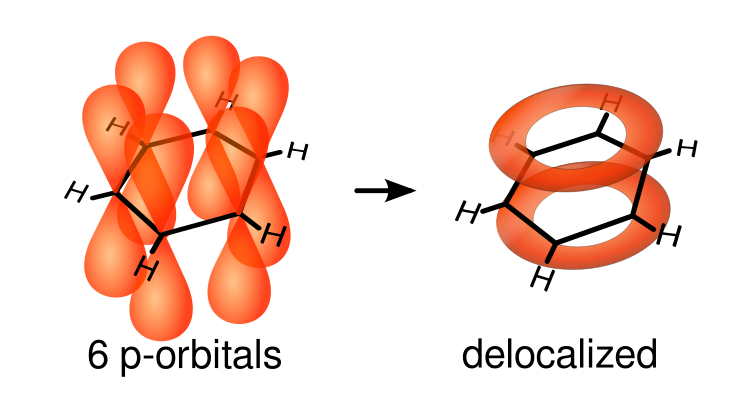
\includegraphics[width=.48\textwidth]{orgSemiconductors/benzene}
\caption{Molecular orbitals of benzene.  The left figure shows the 6 out of plain p$_z$ orbitals, and the right image shows the delocalized $\pi$-bond. \url{https://upload.wikimedia.org/wikipedia/commons/thumb/9/90/Benzene_Orbitals.svg/750px-Benzene_Orbitals.svg.png}}
\label{fig:orgSemi_benzene}
\end{wrapfigure}

To exhibit semiconducting behavior, distributed electrons must exist within the system.\supercite{Neamen1992}
For organic molecules, this is achieved through overlapping p orbitals from carbon.  
Through alternating single and double bonded carbon, hybridized 2p and 2s orbitals form three sp$^2$ orbitals and leave one unhypridized p$_z$ orbital.
These remaining p$_z$ orbitals can interact, forming a $\pi$-bond and delocalizing of the electron cloud, known as \textit{conjugation}.
An example of this is shown for benzene, in Figure \ref{fig:orgSemi_benzene}.

When this conjugation and blending of molecular orbitals occurs, discrete energetic states mix, and resulting in multiple energetic states.\supercite{Kittel2005,Wallis2000}
With more delocalization comes more states resulting in bands of allowed electron energies.
In order to exhibit semiconducting behavior, the resulting bands should result in a set of filled electronic states seperated by a gap from a band of unocuppied states.
For the organic small molecules of interest to this study, delocalization occurs on individual molecules, resulting in less delocalization and thus less dense bands than would be observed in a typical semiconductor, such as silicon or germanium, but the concept remains the same.
In organic molecular semiconductors, the highest occupied molecular orbital (HOMO) and lowest unoccupied molecular orbital (LUMO) reflect the same concept as the valence and conduction bands of inorganic semiconductors, respectively.
The HOMO is filled with electrons and the LUMO is empty in the ground state.
When excited, electrons can be transported through the LUMO levels.
The will result in an electron vacency in the HOMO, known as a \textit{hole}

\section{Charge Transport}

Charge transport in organic semiconductors can take on a variety of behaviors, depending on material and morphology.\cite{Pope1999,Mark1962}
Two regimes of operation are typically expected, being band transport and hopping transport.  
As disorder increases, a shift from band to hopping transport is expected.
Most materials as deposited in our lab are amorphous, so a hopping transport is expected.

\subsection{Band Transport}

Band transport is expected in most atomic crystals, and is thus extensively characterized for inorganic semiconductors.\supercite{Kasap1997}.

\subsection{Hopping Transport}

\section{Excitons}\label{sec:excitons}
\subsection{Singlets and Triplets}


\begin{wrapfigure}{r}{.5\textwidth}
\centering
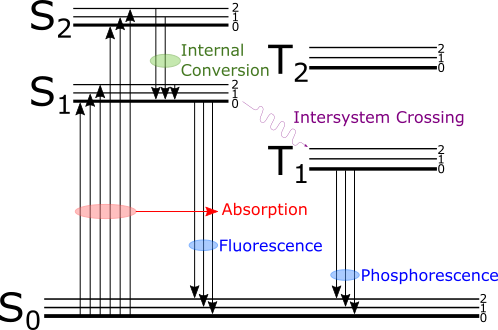
\includegraphics[width=.48\textwidth]{orgSemiconductors/jablonski}
\caption{Simplified Jablonski diagram.}
\label{fig:orgSemi_jablonski}
\end{wrapfigure}


\subsection{Electronic Transitions}
\subsection{Quenching Processes}
\subsection{PL efficiency}





\ifcsdef{mainfile}{}{\printbibliography}
\end{document}
